\documentclass[tikz,border=10pt]{standalone}
\usepackage{tikz}
\usetikzlibrary{arrows.meta, calc}

\begin{document}
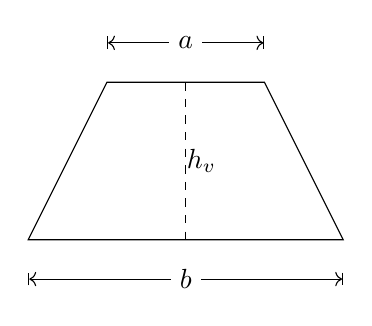
\begin{tikzpicture}

% Define the coordinates for the vertices of the trapezoid
\coordinate (A) at (0,0);
\coordinate (B) at (4,0);
\coordinate (C) at (3,2);
\coordinate (D) at (1,2);

% Draw the trapezoid outline
\draw (A) -- (B) -- (C) -- (D) -- cycle;

% Calculate the midpoint of the top side (DC)
\coordinate (MidTop) at ($(D)!0.5!(C)$);

% Calculate the base of the perpendicular from the midpoint to base AB
\coordinate (BaseOfPerp) at ($(A)!(MidTop)!(B)$);

% Draw the height with dashed line
\draw[dashed] (MidTop) -- (BaseOfPerp);

% Label the height
\node at ($(MidTop)!0.5!(BaseOfPerp)$) [xshift=2mm] {$h_v$};

% Draw and label the bottom side (b)
\draw[|<->|] ([yshift=-0.5cm]A) -- ([yshift=-0.5cm]B) node[fill=white, midway] {$b$};

% Draw and label the top side (a)
\draw[|<->|] ([yshift=0.5cm]D) -- ([yshift=0.5cm]C) node[fill=white, midway] {$a$};

\end{tikzpicture}
\end{document}